\documentclass{article}
\usepackage[margin=1.0in]{geometry}
\usepackage{amsmath, amssymb, mathrsfs}
\usepackage[english]{babel}
\usepackage{graphicx}
\usepackage{enumerate}
\usepackage{listings}
\usepackage{tikz}
\renewcommand{\vec}[1]{\mathbf{#1}}
\newcommand{\floor}[1]{\left\lfloor #1 \right\rfloor}
\newcommand{\ceil}[1]{\left\lceil #1 \right\rceil}

\title{Machine Learning from Data Assignment 11}
\author{Greg Stewart}
\date{\today}

\begin{document}

\maketitle

\subsection*{$k$-NN Rule.}

\begin{enumerate}[(a)]
  \item \textit{Use cross validation with the training set to select the optimal $k$. Plot 
    $E_{CV}$ vs $k$.}

    \includegraphics[width=\textwidth]{3NNECV1.eps}

    From this we select $k = 3$ as the optimal $k$.

  \item \textit{Plot the decision boundary for that $k$. Give the in sample and cross validation
    errors.}

    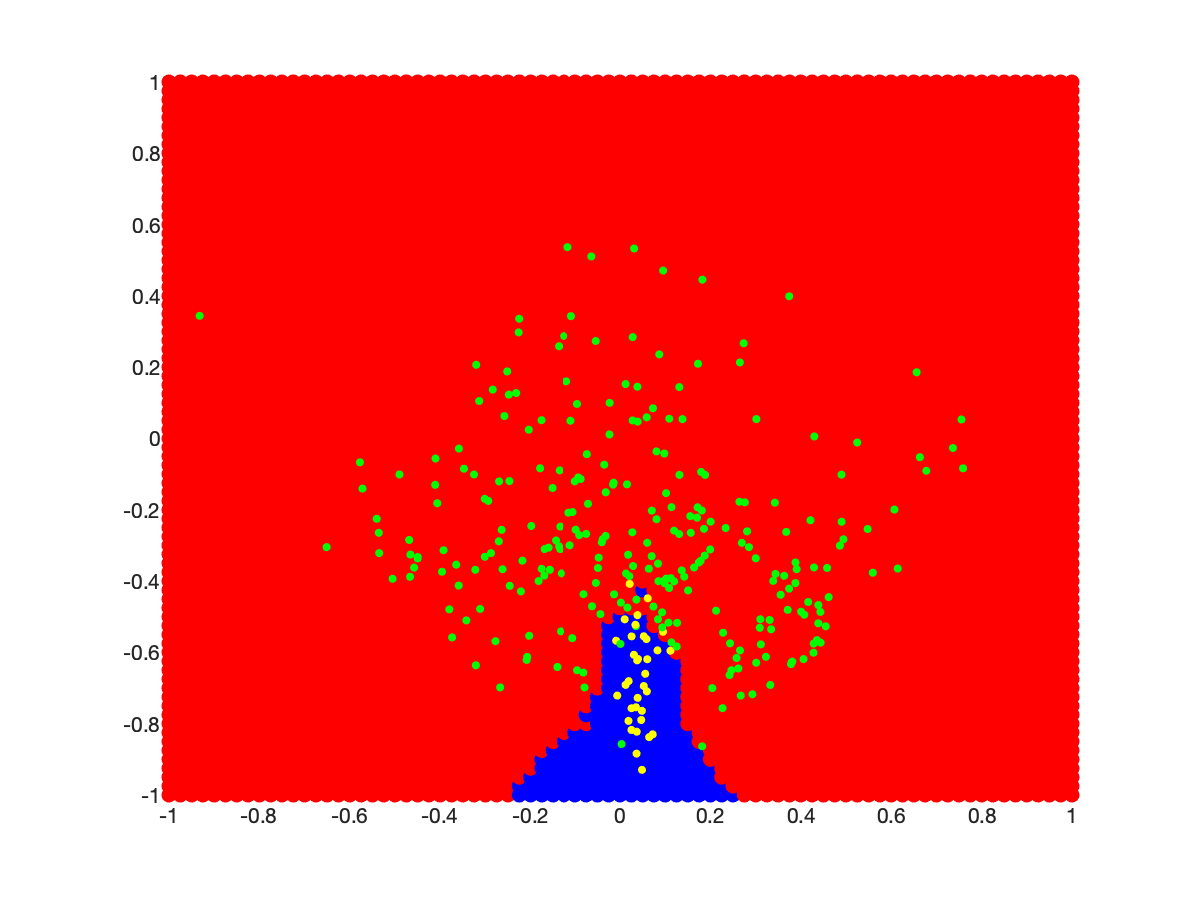
\includegraphics[width=\textwidth]{3NNdecision1.eps}

    The cross validation error is $E_{cv} = .04 = 4\%$.

    The in-sample error is $E_{in} = .06 = 6\%$.

  \item \textit{Give the test error.}

    The test error here is $E_{test} = .0609 = 6.09\%$.

\end{enumerate}

\subsection*{RBF-Network.}

\begin{enumerate}[(a)]
  \item \textit{For RBF with Gaussian kernel, set scale $r = \frac{2}{\sqrt{k}}$ where $k$ is the
    number of centers. Use cross validation with the training set to select optimal number of
    centers $k$. Plot $E_{CV}$ vs $k$.}

    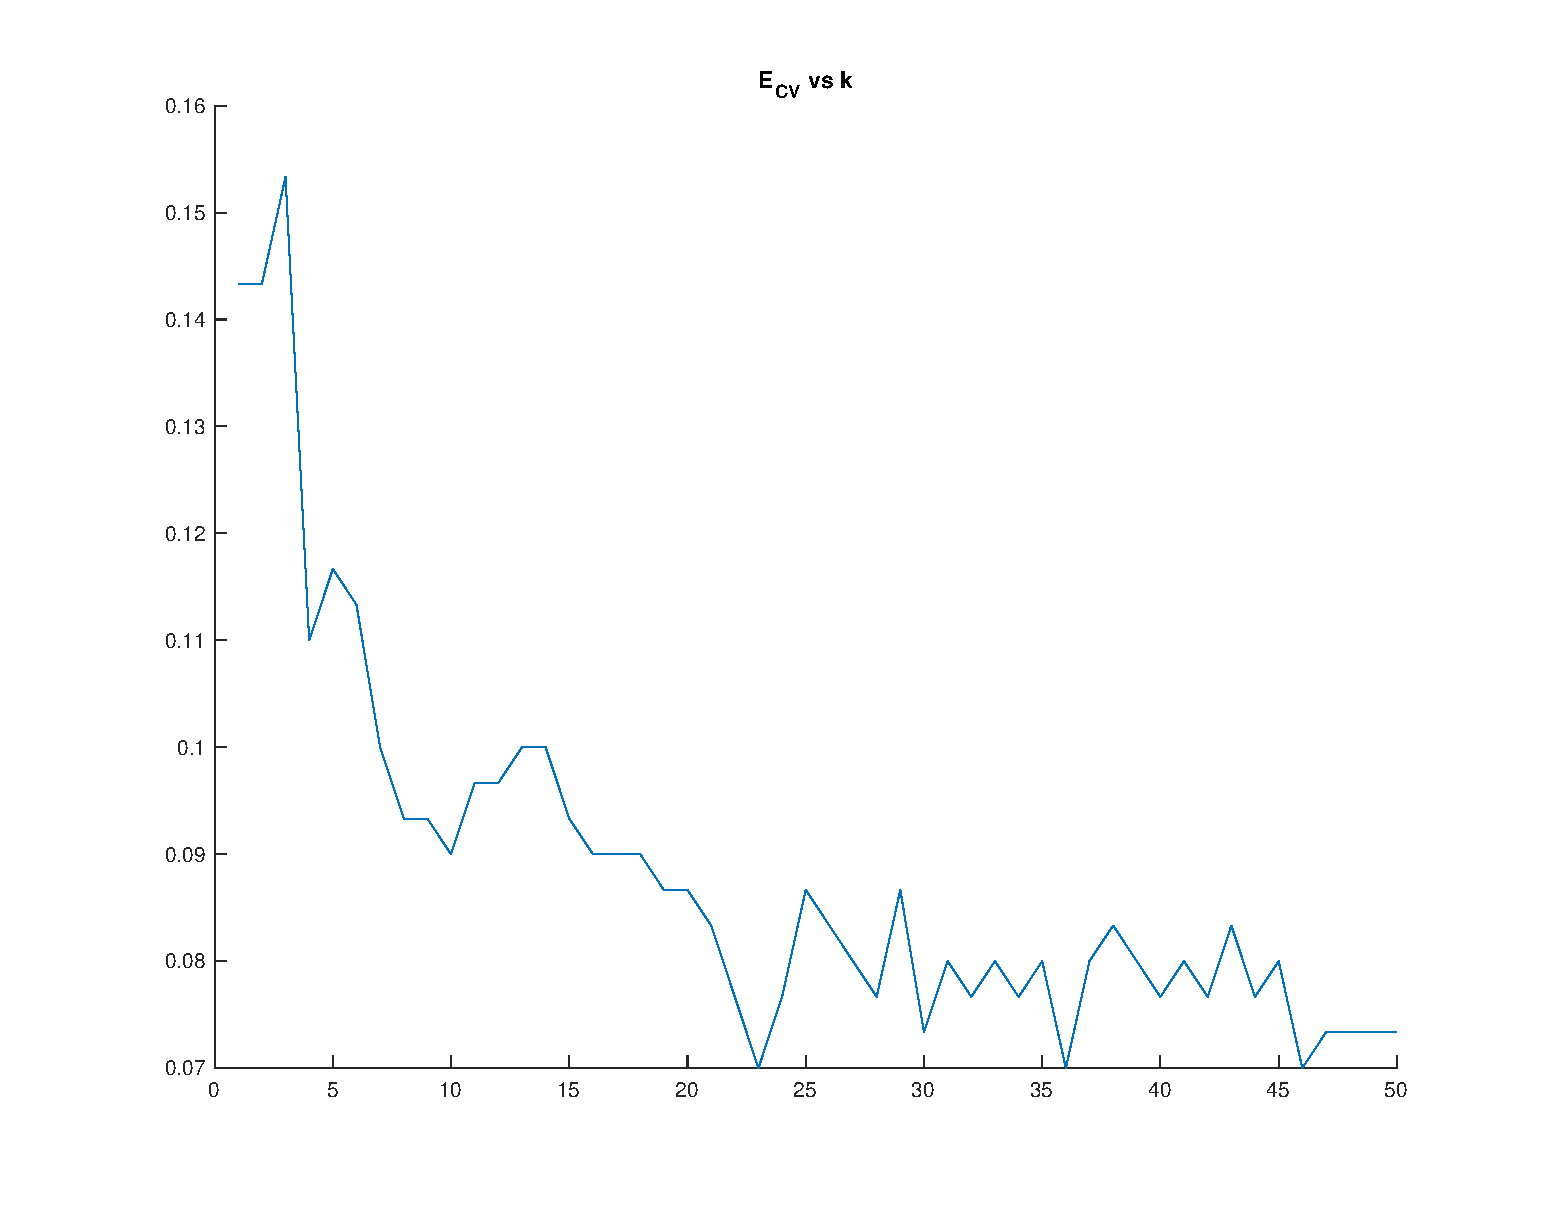
\includegraphics[width=\textwidth]{RBF23ECV.eps}

    The optimal value of $k$ was 23; i.e. there are 23 centers used for the decision boundary.

  \item \textit{Plot the decision boundary for that $k$. Give the in sample error and cross
    validation error.}

    The following boundary was obtained with the pseudo inverse linear regression and a hint of
    regularization.

    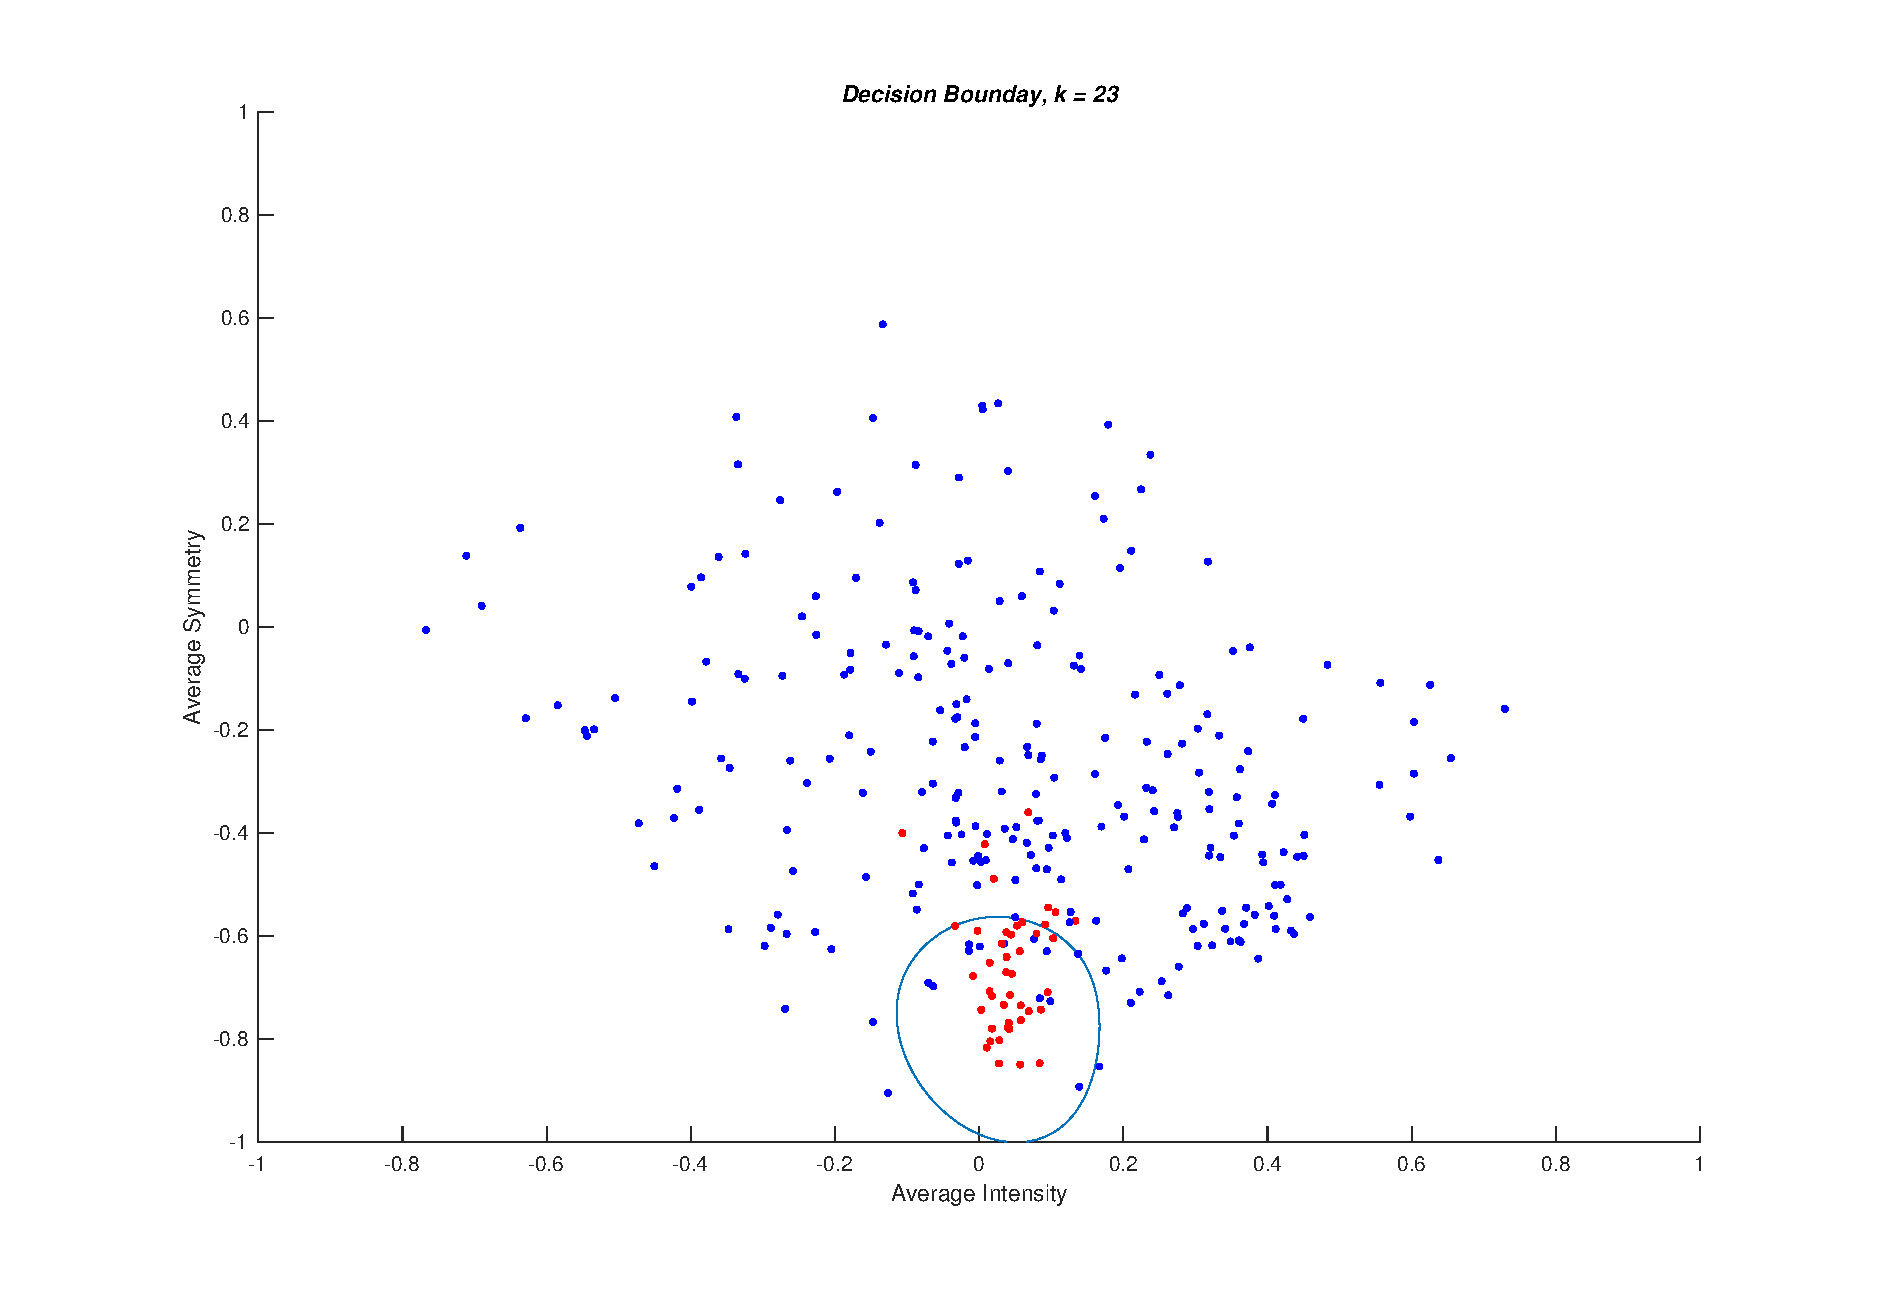
\includegraphics[width=\textwidth]{RBF23.eps}

    The cross validation error for this case was .07, or 7\%.

    The in-sample error $E_{in}$ is .063, or 6.3\%.

  \item \textit{Give the test error.}

    The test error is $E_{test} \approx .062 = 6.2\%$

\end{enumerate}
    
%k = 34 -> Ecv = .06 -> Et = .062569
%k = 24 -> Ecv = .076667 -> Et = .072349
%k = 24 -> Ecv = .05667 -> Et = .066348
%k = 45 -> .06 -> .061903
%k = 11 -> .076667 -> .076017
%k = 20 -> .03 -> .070238
%k = 23 -> .07 -> .062

\subsection*{Linear vs $k$-NN vs RBF-Network.}

\textit{Compare the final test errors from the three attempts done to solve this problem. Make
some intelligent comments.}

Of the three, the $8^{th}$ order Legendre transform has the highest test error, and thus the 
highest $E_{out}$, at 6.7\%. Next smallest, we have the RBF network, with an approximated 
$E_{out}$ of 6.2\%, and the 3-NN boundary, with $E_{out}$ of approximately 6.1\%.

These last two are very similar in $E_{out}$, which is not terribly surprising considering the 
similarity of the methods. The result of the 3-NN rule is in some ways superior as it's about as
good as the RBF network result, but takes significantly less time to compute, thanks to the
simplicity of the calculation. RBF involves much more computation, so it of course takes longer.
However, only pseudo inverse regression with regularization was used for this calculation; the 
result could likely be improved if more work was done, for example by running the pocket 
algorithm. While I haven't computed it here, the improvement from doing so may be worth it.

The result of the $8^{th}$ order transform is the worst of the bunch, and goes to show that
adding complexity and degrees of freedom to the transform does not necessarily increase the
quality of the result. The risk of overfitting is also increased, though regularization helps.
However, the computation is quick, which has benefits. 

\end{document}
